\documentclass[12pt]{article}
\usepackage{fullpage}
\subsectionfont{\fontfamily{phv}\fontsize{13pt}{13pt}\selectfont}
%\newcommand{\var}[1]{\mathit{#1}}
\usepackage[margin=2cm]{geometry}
\usepackage{amsmath}
\usepackage{graphicx}
\usepackage{listings}
\begin{document}
\begin{titlepage}
\newcommand{\HRule}{\rule{\linewidth}{0.5mm}} % Defines a new command for the horizontal lines, change thickness here
\center % Center everything on the page
%----------------------------------------------------------------------------------------
% HEADING SECTIONS
%----------------------------------------------------------------------------------------
\HRule \\[0.4cm]
{ \huge \bfseries Phase 4}\\[0.4cm] % Title of your document
\HRule \\[1.5cm]
\begin{minipage}{0.4\textwidth}
\begin{center} \large
Programming on the Web\\
CSC309H1, Winter 2015\\
\today
\end{center}
\end{minipage}
\vfill % Fill the rest of the page with whitespace
Cody Rosevear, c3roseve\\
999499332\\
\\
Denis Marchin, g3dmarch\\
999061009\\
\\
Farzad Hemmati, c3hemmat\\
999964953\\
\\
Akira Kakkar, g3fol\\
999825541\\
\\
\end{titlepage}
\newpage
\section*{Report}
\begin{enumerate}

\item[0.]

\textbf{Website URL:}
http://104.236.231.174/


\textbf{Summary Of Changes}

-Revised the feature and functionality section to be more descriptive of the user experience expected of the end product.

-Added a section on the rationale of the choice of, and method of integration, of various web technologies.

-Revised the software architecture section in light of the final product.

-Revised the information representation section in light of the final product.

-Revised the project milestones section in light of current developments.

-Added a feature omissions sub-section to the feature and functionality specification section.

-Added the rationale behind the chosen web development technologies.

-Added clarification on testing strategy.

\item[1.] Key Feature and Functionality Specification


\textbf{All pages}

Features:

-Login button

-Register button

-Contact button

-Admin button (if logged in user is an admin)

Description:

On every page there should be a header with the above mentioned buttons, each of which takes the user to the respective page when clicked on.

There is also a footer at the bottom of each page.


\textbf{Homepage}

Features

-Browse button

-Create button

-Search bar

Description:
If logged in, the create button should take the user to the project creation page. If they are not logged in, it should take them to the login page.

The browse button can be used by any user, whether logged in or not.
Similarly, the search bar at the page center can be used by any user, whether logged in or not; it brings the user to the browse page and displays the result of the search.

The rest of the page displays some general information about the site.

\textbf{Register Page}
Features:

-Name box

-Email box

-Password box

-Re-enter password box

Description:
The user should be able to register via the given form.
Blank fields, emails without proper format, mismatched passwords, and usernames that are already taken should result in prompts to the user to correct any issues.
Once the form is submitted, the user should be redirected to the home page, but with a status of logged in.

\textbf{Login Page}
Features:

-Email box

-Password box

-Login Issues box

Description:
From here the user should be able to log in by providing the correct username(email address) and password.

There should be a button the user can press if they are having issues logging in. This brings the user to the contact page in order to get help resolving their log in issues.

There should also be an option to reach the register page if the user does not yet have a profile.

\textbf{Contact Page}

Features:

-Name box

-Email box

-Message box

Description:
Provided that the user has filled in all of the blank fields and supplied a valid email address they should be able to send a message to the site staff.

\textbf{Edit Profile Page}

Features:
-Name box

-Password and confirm-password boc

-Image upload section

-Bio text area

Description:
Here the user should be able to update their name, profile picture, biography and password information.

\textbf{Profile Page}

Features:
-Profile picture

-Edit button (if the profile belongs to the logged in user)

-Like/Dislike function (for members in the same community)

-Name

-Community members list

-Reputation score

-Initiated projects list

-Project contribtuions list

-Bio

-Date joined

Description:
The profile should contain all of the basic public information for a given user. The name and biography (detailing all the history, as well as relevant skills and experience of the user), should be alterable via the edit button.
The date joined, and reputation score are not alterable by the user, but determined automatically and by other user's in the site who are friends with the user whose profile is being viewed.
Individuals become friends with anyone who is already associated with a particular project, and anyone who makes or contributes to a project is said to be associated with it.
The profile should include a list of community members, which is a master list of all of the friends the user has in every community.
The reputation score will be a numeric value computed by summing the total number of likes and subtracting the total number of dislikes.
Only user's who are members of the same community can vote on eachother's profiles, and they can do so only once.
Finally, there should also be a list of the projects initiated by the user, as well as a list of those to which the user has made contributions. The former should include the date of creation of the project while the latter should include the amount of money contributed for each donation.

\textbf{Browse Projects Page}

Features:
-Category menu

-Category button to filter by project categories (within a user's communities)

-Project info box

Description:
The use should be able to filter out the projects according to the pre-specified categories provided.
Each of the projects shown as a result of filtering should display some basic information about the project, such as the title, the funding goal, the current amount of funding for each project, the number of likes/dislikes as well as the project name, creator, and description.

\textbf{Create/Edit project page}

Features:
-Project name box

-Category drop down selection

-Funding goal box

-Description box

Description:
This page should allow the user to create a new project by specifying the project name, cateogry, funding goal, and a description. Blank fields should prompt the user to fill them in, and the funding goal must be positive.

Users must be logged in in order to create a new project. Attempting to create a project without logging in should redirect the user to the log in page, where they can then log in or proceed to the register page if they do not have an account.

\textbf{Project Info Page}

-Project video and or image

-Project description

-Creator name

-Date created

-Funding goal

-Current funding amount

-Fund button

-Edit/delete button (if the current user is the project creator)

-Testimonial section

Description:
This is the on-line pitch that other community members see when deciding to fund a project.
It should include a video or representative image of the project as well as a written description detailing the  project and its founders.
Other users within the community should be able to rate the project by likin/disliking it, as well as leave testimonials concerning the project. The funding funding page should be accessible from this point, and all of the information pertaining to the funding goal, such as how much they currently have, and how much is still needed to reach their goal should be present.
Finally, provided the user viewing the current project is also its creator, the edit and delete project buttons should be present. The delete project button should prompt the user for confirmation before actually deleting the given project, so as to minimize accidental deletions.


\textbf{Fund Page}

-Funding amount entry box

-Payment details input box

Description:
Users should be able to enter their payment information details as well as the amount of money they want to donate to
the given project.

\textbf{Administrator Page}

Features:
-Total number of projects

-Total number of projects funded

-Average time to reach a funding goal

Description:
The admin page will provide the administrator with the capacity to view an important number of pre-specified statistics. These include the total distribution of projects by category, the total number of projects and users, as well as a breakdown of the funding status distribution among projects, where the funding status of any given project can be in one of three states: unfunded, partially funded, and completely funded.
Moreover, this page will allow current administrators to add other users to the administrator list.
Finally, administrator's will also have the capacity to edit and/or delete any projects irrespective of whether they created it or not.

\textbf{Omissions}

Payment verifier: 

Originally we had intended to integrate some sort of third party payment verification in the back end of the funding page. However, as progess developed, we realized that a live payment verifier was not actually part of the project specification as provided in the hand out, and so we decided to simply implement the front end of the funding page without any actual verification.

The credit card page still allows for live data to be added to the website projects, it is, however, not necessary that the user provide a valid credit card, and their is no charging of any such credit card. Instead, the data provided on the input form is submitted directly to the database to simulate the necessity of managing credit card transactions as they would effect the project.

Ideally, if implemented, validation and exchange of funds would be done via integrating our website with a third party service, such as PayPal. 


\begin{figure}[ht!]
\centering
\includegraphics[width=200mm]{flowchart1.pdf}
\caption{Website Flowchart \label{overflow}}
\end{figure}


\item[2.] Project Plan

\textbf{General protocol}

Communication Methodology: Weekly meetings will occur on Wednesday's before class to discuss any issues related to development and write the weekly report. Moreover, Skype and Facebook will serve as methods of contact for resolving any immediate issues.

Team Roles: These will be contingent on the phase of development, and assigned for the given week at each weekly meeting. That is, the responsibilites of each team member will be decided on a weekly basis.

Problem resolution: All decisions are made democratically by vote.

Hosting of Source: GitHub

\textbf{Milestones}

Note 1: The following schedule is ordered according to the perceived dependencies of the various features of the website. First the raw skeletons, then the database underlying all of the website information, followed by suitable integration between the database and web pages so that they display all of their content properly. Then, the more dynamic functionality is built weekly on top of this static base. 

Week1: Page skeletons, links, and basic styling

Week2: Central Database design and query development for all pages that use said database.

Week3: Project/Community/Profile page information is integrated with the database such that the pages display accurately.

Week4: Search functionality for all types of pages is operational.

Week5: Additional project and profile page development

Week6: Review System and Payment System

Week7: Admin Analytics

Week8: Additional Debuggging and Development Overflow

\item[3.] Software Architecture, and Technology Stack
\begin{figure}[ht!]
\centering
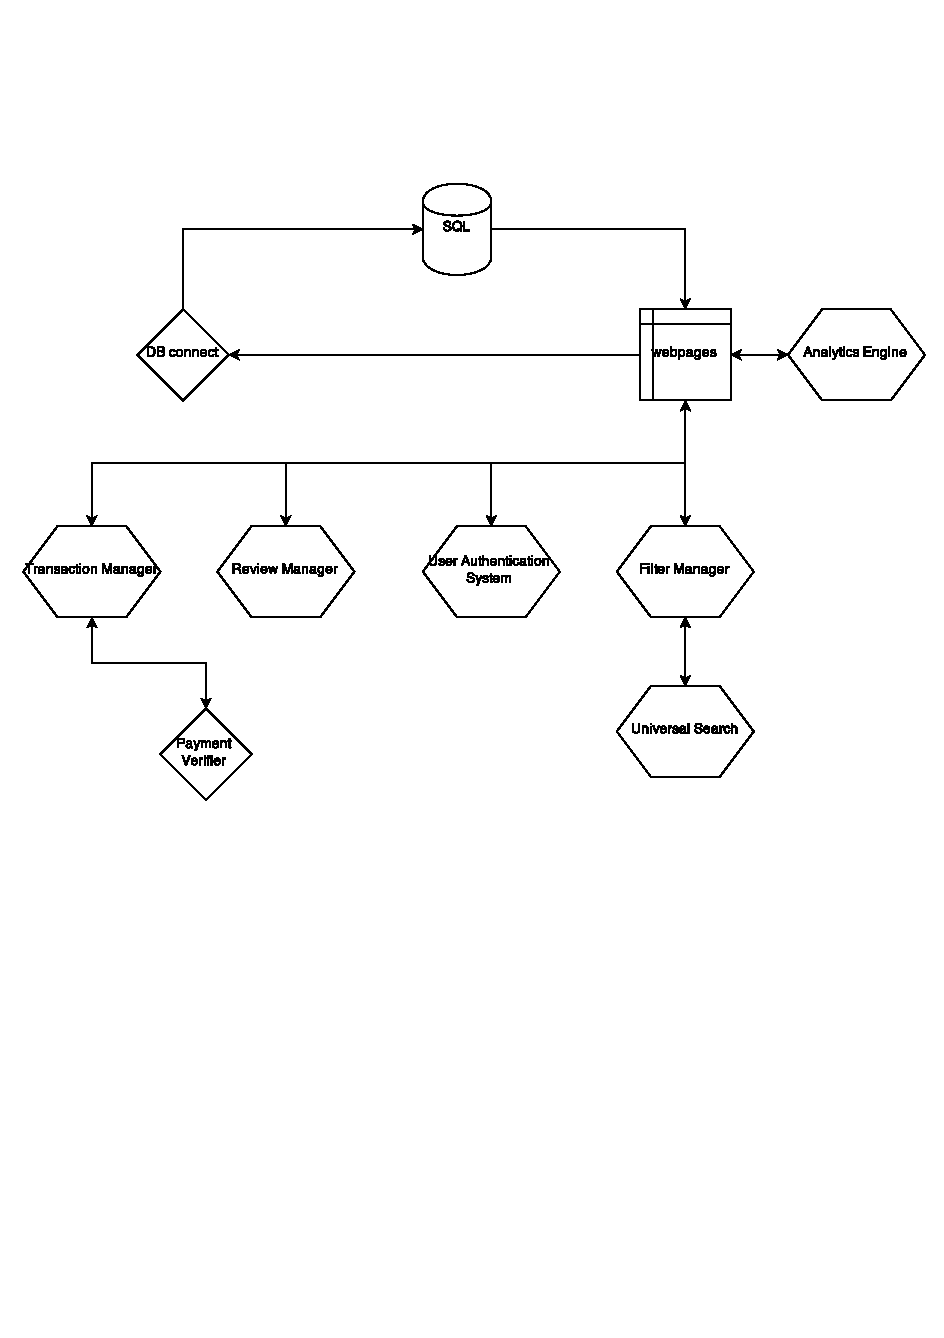
\includegraphics[width=150mm]{swag.pdf}
\caption{Software Components \label{overflow}}
\end{figure}

Technology Decisions And Rationale:

We are using PHP as our server side technology for a number of reasons: its ease of integration with HTML, it's incorporation in the XAMPP/MAMPP development environment, as well as the fact that it has a large user base, and as such there is a good amount of third party library support for accomplishing many tasks, such as mailing, graphics, etc... Moreover, since we are not particularly concerned with scalability at this point, we are not concerned so much with issues of language perfromance, but rather, given the time constraints, how well that language will allow us to develop and prototyp rapidly. In this respect, PHP is a good choice. 

For the front end we will be using HTML solely for structure and CSS for presentation, so as to allow for a greater separation of concerns. This will make the code organized, and easier to maintain and modify in light of new developments as the project progresses, since we will be able to change the style or structure uniformily without impacting the other. With respect to CSS, we have also opted to use Bootsrap3 to provide us with a general stylistic template upon which to build. As above, this decsion to use a framework is motivated by the desire for rapid development at the cost of a greater degree of overall flexibility.

For our RDBMS we have chosen to use MySQL. As above, this is largely due to the fact that it is capable of easy integration with PHP via the phpMyAdmin interface provided in the XAMPP/WAMPP development environment. Moreover, MySQL is familiar to all members of the team, which is an important facet to consider given that this is likely to reduce the overall learning curve and improve weekly productivity, which is important given the time constraints associated with the project. Finally, MySQL is well known for both its popularity and its quality, both of which are important factors we considered in choosing it. The former provides, again, a large user base from which to draw support when learning, and the latter provides us with an assurance that the data transactions subserving our website will meet at least a minimal degree of efficiency (even though we are not so much concerned with performance at this point as rapid development).


Software Architecture:


We will have a central MySql database which keeps track of all the data associated with each of the various webpages. This will be the central repository from which all of the dynamic webpages will request information from when displaying webpages to users. It will also serve as the storehouse for transaction logging of all kinds, including funding transactions ad vote transactions pertaining to both projects and profiles. We chose MySQL because of everyone's familiarity with it, it's integration with XAMPP/MAMPP

We will also have a database connector module that will be used by all of the webpages, so as to avoid code duplication.

All of the individual manager components are subsets of the functionality of the webpages themselves, and are therefore connected to the central database inasmuch as the webpages are connected to it.

The filter manager is the core software component that sub-serves all of the search functionality of the browse pages (both the category filter and the general search box).

The review manager provides the functionality to each project page which allows for funders to comment on projects as well as the reviews of other funders. It will need to be decomposed into both a rating system as well as a comment system.

The admin analytics component sub-serves the unique features of the admin view. It interacts with the central database, using the data stored there to compute statistics.

Finally, the user authentication system will be utilized wherever any kind of authentication is necessary. Since the process should generally be the same irrespective of the reason for authentication, it can be modularized.


\item[4.] Information Representation\\
Relations:

users(\underline{userid} date, name, email, password, reputation, bio, admin)\\
transactions(\underline{transactionID}, pID, date, user, amountfunded)\\
projects(\underline{pId}, title, description, date, creator, goal, funded, category, likes, dislikes)\\
profilevotes(\underline{voter, votee})\\
friends(\underline{userid, pid})\\
comments(\underline{cid}, pid, userid, comment, date)\\

Constraints:

projects(creator) \subseteq users(userid)\\
transactions(user) \subseteq users(userid)\\
profilevotes(voter) \subseteq users(userid)\\
profilevotes(votee) \subseteq users(userid)\\
friends(userid) \subseteq users(userid)\\
comments(userid) \subseteq users(userid)\\
friends(pid) \subseteq projects(pid)\\
transactions(pid) \subseteq projects(pid)\\
projects(creator) \subseteq users(email)\\

Relations And Website Interaction:

users:
This relation will be used to keep track of the authentication credentials for each user. It will also store the user profile data that is dynamically applied to a static profile page template when the user is viewing a particular profiel. This relation will also store information used by the project info page to specify details about a projects creator. Like the profile page, this data will by accessed dynamically based on the project and then applied to a static project template page.

transactions:
This relation will store the donations that individual users make via the project info page. This data will be used by the profile page code to extract the contributions of the user whose profle is currently being viewed.

projects:
This relation will store all of the information that is to be dynamically loaded into the static project page template of individual projects. Moreover, it will also be utilized by the information displays that are the result of the search functionality provided by the category filter and project search bar. Finally, this information will interact directyl with the profile page, in that the profile page code will use this relation to determine which projects to display as having been created by the user of the current profile being viewed.

profilevotes:
This relation will keep track of which members of a community have voted on other members of a commuunity. This data will be used to determine whether or not the like/dislike function should be displayed on the profile page that is currently being viewed, provided that the user of the current profile is a friend of the currently logged on user.

friends:
This relation will contain all of the members of a community. Since a community is defined via association with a given project, any user whose id is contained within a tuple that also contains the id of that project is considered friends with every other member of the community defined by that project.

The data in this relation will be used by the profile page to determine who are the friends of the user represented by the current profile page. It will also be used by the profile page to determine whether or not the like/dislike function used to rate profiles should be available to the currently logged in user viewing the current profile.

comments:
This relation will be used by the project info page to render a list of testimonials pertaining to the current project.

\item[5.] Test Strategy and Test Plan

Just as project initiators on this site will test their ideas and creations, we have been testing the website. Hard staff responsibilities are assigned on a weekly basis. All team members are responsible for testing the website. Website builders are expected to do some level of testing as they create a feature. GitHub is used to store the group�s file assets. When a feature has been sufficiently tested, the corresponding files are committed to the shared repository. Heavy testing of the feature from as many angles as possible will be completed nearer the end of the project phase. When all pages and features have been created, the testing will go into beta. During the beta phase of development, the team will shift their focus from content creating, to content testing. 

Basic testing is done in a timely manner, and before starting new feature additions. Record keeping of testing takes place. Untested, and therefore possibly broken additions, should be marked as such in the commit message. Features that have been tested to work properly will also be marked as such in the commit message. At our weekly meetings, team members are expected to give a report update on what testing they have completed that week, and we will distribute the new testing tasks.\\

The development team is employing an array of testing strategies to ensure a properly functioning website. The user interface needs testing. We want the website to feel intuitive and easy to use. We do not want to discourage users by having a steep learning curve. As the webpages are built, the layout and navigation will be tested for user friendliness. The website will be tested in the most popular web browser programs: Internet Explorer, Firefox, Safari, and Chrome. Layout may be displayed differently upon different browsers, and we want to ensure an appealing style across all possible browsers the user may use. 

Near the end of the project phase, we will elicit our peers to test the website for ease of use. The major testing is for the databases. We are using phpMyAdmin for database management. Queries are tested for correctness. We ensure data is received and is outputted correctly. Error messages are coded-in to alert testers and users of foreseeable problems, such as not being able to connect to the server. Security is an extremely important element to test. We are storing sensitive information in our database, such as passwords and emails, and have a responsibility to protect the data of our users. The databases are currently populated with dummy data in order to simulate the site being operational, with many users, communities, projects, and their interactions. Common security flaws are assessed and tested against, such as SQL injection. 

Data validation is extensively tested, with test cases to guarantee only appropriate data in accepted. Unit testing will be used to test individual components to simplify the scope of problems. Examples of units tested are the header and footer, which are now incorporated on each page after being tested to work on their own. Users will be able to search for project using various categories. Unit testing will be used to test the site�s search function. Each type of search will be tested, and will use a test database to search against. Proper code layout is important for clarity and is a best practice. Having a uniform standard for the code layout is especially important when working in a multi-person group. Code is tested in a style validator such as W3C Markup Validator. Code layout will also be evaluated by the team as each member is to look over each line before the final submission. Development team members are free to use any program to write page code in, such as Sublime Text Editor. 

Code is encouraged to be written in an IDE with a comprehensive debugger, such as Netbeans. Code written outside of an IDE can still later be tested in one. XDebug from NetBeans IDE is used to test PHP. Using XDebug, the developer can cause pauses at breakpoints and retrieve information about the current program state, such as the values of the program variables. As the team does not have sufficient funds for professional software, we are relying on open source or free-to-use testing methods. Our webpage contains a �Contact us� option on every page, allowing users to report any problems they might encounter while using the website. Creating not only a working site, but an enticing one, through the process of thorough testing will give this site the potential for popularity.

\end{enumerate}
\end{document}
